\chapter{Betriebssystemübersicht}

Zu Begin des Projektes standen die beiden Betriebssysteme OpenWRT und Bananian zur Verfügung.
Außerdem gab es den Vorschlag des Vorgängerprojekts, zusätzlich das Projekt auch mit dem Betribssystem IPFire durchzuführen.
Die Nutzung der einzelnen Betriebssysteme fiel sehr unterschiedlich aus, da die implementierten Funkionen und der Stand der Entwicklung sich stark von System zu System unterschied.

\section{OpenWRT}
OpenWRT ist ein Betriebssystem, das für eingebettete Geräte wie Wlan Router enwickelt wurde.
Das System wird über ein Webinterface angepasst und unterscheidet sich stark zu den anderen im Projekt verwendeten Betriebssystemen.
Durch diese Unterschiede wurden nur enzelne Teile des Projektes auf OpenWRT umgesetzt.

\section{IPFire}
\begin{wrapfigure}{r}{5cm}
\centering

\includegraphics[width=3.5cm]{pictures/Jakob/IPFire}
\caption{IPFire Logo}
Quelle: \cite{fire1}
\end{wrapfigure}
Das Betriebssystem IPFire ist darauf ausgelegt, als Router genutzt zu werden, wobei das Augenmerk auf der implementierung einer Firewall oder eines VPN Gateways liegt.
Das vorgehende Projekt hatte dieses Betriebssystem als Alternative vorgeschlagen, weshalb wir dieses System als Aternative untersucht haben.
Zwei Abbilder für den Betrieb auf ARM Prozessoren stehen auf der Webseite des Betriebssystems bereit. \cite{fire} \\
Bei beiden Abbildern stellte sich allerdings herraus, dass die HDMI Schnittstelle nicht unterstützt wird.
Auch eine Verbindung über SSH nicht möglich ist, da IPFire auf die Konfiguration über ein Webinterface ausgelegt ist.
Eines der beiden Abbilder ist auf die Konfiguration über eine Serielle Schnittstelle ausgelegt. Da uns aber für diese Schnittstelle keine Wekzeuge und Adapter bereitstehen, haben wir auch von dieser Option abgelassen.\\

\newpage
\section{Bananian}
\begin{wrapfigure}{r}{5cm}
\centering

\includegraphics[width=3cm]{pictures/Jakob/Bananian}
\caption{Bananian Logo}
Quelle: \cite{bananian1}
\end{wrapfigure}
Der Banana Pi R1 wird von dem Betribssystem Bananian vollständig unterstützt. Dieses Betriebssystem basiert auf Debian 8 und nutzt das Debian Jessie armhf repositorie. \cite{bananian}\\
Neben OpenWRT wurde das Projekt mit Bananian gestartet. Da die Weiterentwicklung von Bananian am 2.4.2017 eingestellt wurde haben wir uns einschieden auf das Betriebssystem Armbian zu wechseln. \cite{bananian2}

\section{Armbian}
\begin{wrapfigure}{r}{5cm}
\centering
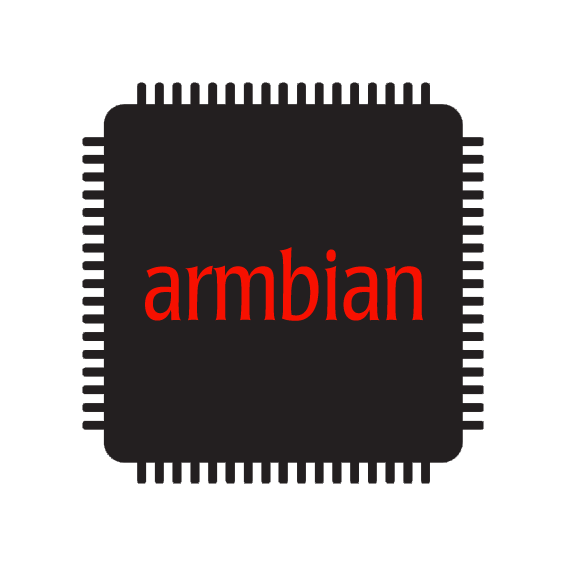
\includegraphics[width=3.5cm]{pictures/Jakob/Armbian}
\caption{Armbian Logo}
Quelle: \cite{armbian}
\end{wrapfigure}
Wie auch Bananian basiert Armbian auf Debian Jessie, das speziell für ARM Prozessoren entwickelt wurde. Dieses Betriebssystem haben wir gewählt, da es Bananien stark ähnelt, im Gegensatz zu Bananian aber weiterentwickelt wird und damit auch in gewissem Maße für die Zukunft gewappnet ist. Außerdem unterstützt es alle Funktionen die für das Projekt benötigt werden. \cite{armbian1}







